\chapter{Lec 15 - Dealing with Uncertainty II}

\section{Conditional independence}
The notion of independence provides a clue of how we can simplify expressions, but it needs refining. It would be nice if $Toothache$ and $Catch$ were independent, but they are not: if the probe catches in the tooth, then it is likely that the tooth
has a cavity and that the cavity causes a toothache. These variables \textit{are} independent, however, \textit{given the presence or the absence of a cavity}.  Each is directly caused by the cavity, but neither has a direct effect on the other: toothache depends on the state of the nerves in the tooth, whereas the probe’s accuracy depends on the dentist’s skill, to which the toothache is irrelevant. Mathematically, this property is written as:
\[\textbf{P}(toothache \land catch | Cavity) = \textbf{P}(toothache | Cavity)\textbf{P}(catch | Cavity) .\]
This equation expresses the \textbf{conditional independence} of $toothache$ and $catch$ given $Cavity$.
The general definition of conditional independence of two variables $X$ and $Y$ , given a third variable $Z$, is
\[\textbf{P}(X, Y | Z) = \textbf{P}(X | Z)\textbf{P}(Y | Z)\]
In the dentist domain, for example, it seems reasonable to assert conditional independence of the variables $Toothache$ and $Catch$, given $Cavity$:
\[\textbf{P}(Toothache, Catch | Cavity) = \textbf{P}(Toothache | Cavity)\textbf{P}(Catch | Cavity)\]
Notice that this assertion is somewhat stronger than the previous one, which asserts independence only for specific values of $Toothache$ and $Catch$.\\\\
Equivalently, conditional independence may be stated as:
\[\textbf{P}(X | Y,Z) = \textbf{P}(X |Z)\]
\begin{center}
    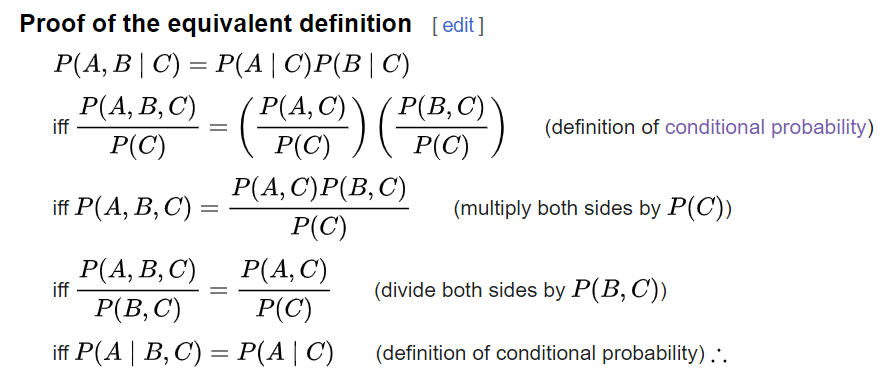
\includegraphics[scale=0.8]{images/proof cond prob.png}
\end{center}
We have shown that absolute independence assertions allow a decomposition of the full joint distribution into much smaller pieces. It turns out that the same is true for conditional independence assertions. For example, we can write out the joint distribution $\textbf{P}(Toothache, Catch, Cavity)$ using the product rule as follows:
\[\textbf{P}(Toothache, Catch, Cavity) = \textbf{P}(Toothache, Catch | Cavity)P(Cavity) \]
Then, we can apply the conditional independence of $Toothache$ and $Catch$, given $Cavity$:
\[= \textbf{P}(Toothache | Cavity)\textbf{P}(Catch | Cavity)\textbf{P}(Cavity)\]
In this way, the original large table is decomposed into three smaller tables. The original table has seven independent numbers ($2^3 = 8$ entries in the table, but they must sum to 1, so 7 are independent). The smaller tables contain five independent numbers. Going from seven to five might not seem like a major triumph, but the point is that, for $n$ symptoms that are all conditionally independent given $Cavity$, the size of the representation grows as $O(n)$ instead of $O(2^n)$.\\\\
That means that conditional independence assertions can allow probabilistic systems to scale up; moreover, they are much more commonly available than absolute independence assertions.

\section{Bayes' Rule}
The product rule we defined before can actually be written in two forms:
\[P(a \land b) = P(a | b)P(b) \,\,\,\, \text{and} \,\,\,\, P(a \land b) = P(b | a)P(a)\]
Equating the two right-hand sides and dividing by $P(a)$, we get
\[P(b|a) = \frac{P(a|b)P(b)}{P(a)}\]
This equation is known as \textbf{Bayes’ rule}. This simple
equation underlies most modern AI systems for probabilistic inference.\\\\
The more general case of Bayes’ rule for multivalued variables can be written in distribution form:
\[\textbf{P}(Y|X) = \frac{\textbf{P}(X|Y)\textbf{P}(Y)}{\textbf{P}(X)} = \alpha \textbf{P}(X|Y)\textbf{P}(Y)\]
It allows us to compute the single term $P(b | a)$ in terms of three terms: $P(a | b)$, $P(b)$, and $P(a)$. Bayes’ rule is useful in practice because there are many cases where we do have good probability estimates for these three numbers and need to compute the fourth. Often, we perceive as evidence the effect of some unknown cause and we would like to determine that cause. In that case, Bayes’ rule becomes:
\[P(cause|effect) = \frac{P(effect|cause)P(cause)}{P(effect)}\]
The conditional probability $P(effect | cause)$ quantifies the relationship in the causal direction, whereas $P(cause | effect)$ describes the diagnostic direction.\\\\
For example, a doctor knows that the disease meningitis causes the patient to have a stiff neck, say, 70\% of the time.  The doctor also knows some unconditional facts: the prior probability that a patient has meningitis is 1/50,000, and the prior probability that any patient has a stiff neck is 1\%. Letting $s$ be the proposition that the patient has a stiff neck and $m$ be the proposition that the patient has meningitis, we have:
\[P(m|s) = \frac{P(s|m)P(m)}{P(s)} = \frac{0.7 \times 1/50,000}{0.01} = 0.0014\]
That is, we expect less than 1 in 700 patients with a stiff neck to have meningitis. We can avoid assessing the prior probability of the evidence (here, $P(s)$) by instead computing a posterior probability for each value of the query variable (here, $m$ and $\neg m$):
\[\textbf{P}(M | s) = \alpha <P(s | m)P(m), P(s | \neg m)P(\neg m)> .\]
Thus, to use this approach we need to estimate $P(s | \neg m)$ instead of $P(s)$. There is no free lunch, sometimes this is easier, sometimes it is harder.\\\\
What happens when we have two or more pieces of evidence? For example, what can a dentist conclude if her nasty steel probe catches in the aching tooth of a patient?
\[\textbf{P}(Cavity |toothache \land catch)\]
We can try using Bayes’ rule to reformulate the problem:
\[\textbf{P}(Cavity |toothache \land catch) = \alpha \textbf{P}(toothache \land catch | Cavity) \textbf{P}(Cavity) . \]
For this reformulation to work, we need to know the conditional probabilities of the conjunction $toothache \land catch$ for each value of $Cavity$. That might be feasible for just two evidence variables, but again it does not scale up. If there are $n$ possible evidence variables (X rays, diet, oral hygiene, etc.), then there are $2^n$ possible combinations of observed values for which we would need to know conditional probabilities.\\\\
If we apply the conditional independence of $Toothache$ and $Catch$, given $Cavity$, it becomes:
\[= \alpha \textbf{P}(toothache|Cavity)\textbf{P}(catch|Cavity)\textbf{P}(Cavity)\]
As we said before, using this simplification, the size of the representation grows as $O(n)$.\\\\
In general, if we want to estimate
\[\textbf{P}(Cause | Effect_1, ..., Effect_n)\]
We can use the Bayes' rule to reformulate the problem as:
\[= \alpha \textbf{P}(Effect_1, ..., Effect_n | Cause) \textbf{P}(Cause)\]
However, it is computational unfeasible to compute $\textbf{P}(Effect_1, ..., Effect_n | Cause)$, therefore we need to rely on some simplification. For example, if we assume that all the effects are conditionally independent, given the cause, i.e, $\textbf{P}(Effect_1, ..., Effect_n | Cause) = \prod_i \textbf{P}(Effect_i| Cause)$, we can express the problem as:
\[\textbf{P}(Cause | Effect_1, ..., Effect_n) = \alpha \textbf{P}(Cause) \prod_i \textbf{P}(Effect_i | Cause) \]
Formally, the full joint distribution can be written as:
\[\textbf{P}(Cause, Effect_1, ..., Effect_n) = \textbf{P}(Cause) \prod_i \textbf{P}(Effect_i | Cause)\]
Such a probability distribution is called a \textbf{naive Bayes model}, “naive” because it is often used (as a simplifying assumption) in cases where the “effect” variables are not actually conditionally independent given the cause variable.  In practice, naive Bayes systems can work surprisingly well, even when the conditional independence assumption is not true.

\section{The Wumpus World Revisited}
We can combine of the ideas in this chapter to solve probabilistic reasoning problems in the wumpus world.  Uncertainty arises in the wumpus world because the agent’s sensors give only partial information about the world.
\begin{center}
    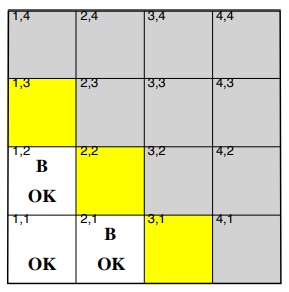
\includegraphics[]{images/Wumpus-probs.png}
\end{center}
For example, the figure above shows a situation in which each of the three reachable squares, $[1,3], [2,2]$, and $[3,1]$, might contain a pit. Pure logical inference can conclude nothing about which square is most likely to be safe, so a logical agent might have to choose randomly. We will see that a probabilistic agent can do much better than the logical agent.\\\\
Our aim is to calculate the probability that each of the three squares contains a pit.  step is to identify the set of random
variables we need:
\begin{itemize}
    \item We want one Boolean variable $P_{ij}$ for each square, which is true iff square $[i, j]$ actually contains a pit.

    \item We also have Boolean variables $B_{ij}$ that are true iff square $[i, j]$ is breezy. We include these variables only for the observed squares, in this case, $[1,1], [1,2],$ and $[2,1]$.
\end{itemize}
The next step is to specify the full joint distribution:
\[\textbf{P}(P_{1,1},...,P_{4,4}, B_{1,1}, B_{1,2}, B_{2,1})\]
Applying the product rule, we have
\[= \textbf{P}(B_{1,1}, B_{1,2}, B_{2,1} | P_{1,1},...,P_{4,4})\textbf{P}(P_{1,1},...,P_{4,4}) \]
The first term is 1 if the breezes are adjacent to the pits and 0 otherwise. The second term is the prior probability of a pit configuration. Each square contains a pit with probability 0.2, independently of the other squares; hence,
\begin{equation}
    \textbf{P}(P_{1,1},...,P_{4,4}) = \prod_{i,j = 1,1}^{4,4}\textbf{P}(P_{i,j})
\end{equation}
For a particular configuration with exactly $n$ pits, $P(P_{1,1},...,P_{4,4}) = 0.2^n \times 0.8^{16-n}$\\\\
We know the following facts:
\begin{itemize}
    \item $b = \neg b_{1,1} \land b_{1,2} \land b_{2,1}$

    \item $known = \neg p_{1,1} \land \neg p_{1,2} \land \neg p_{2,1}$
\end{itemize}
We are interested in answering queries such as $\textbf{P}(P_{1,3} | known, b)$: how likely is it that $[1,3]$ contains a pit, given the observations so far?\\\\
To answer this query, we can follow the standard approach summing over entries from the full joint distribution.  Let $Unknown$ be the set of $P_{i,j}$ variables for squares other than the $Known$ squares and the query square $[1,3]$. Then we have:
\[\textbf{P}(P_{1,3} | known, b) = \sum_{unknown} \textbf{P}(P_{1,3}, unknown, known, b)\]
Basically, it sums over all the possible combinations of the values of the unknown squares. There are 12 unknown squares; hence the summation contains $2^{12} = 4096$ terms.  In general, the summation grows exponentially with the number of squares.\\\\
Surely, one might ask, aren’t the other squares irrelevant? How could $[4,4]$ affect whether $[1,3]$ has a pit? Indeed, this intuition is correct. Let $Frontier$ be the pit variables (other than the query variable) that are adjacent to visited squares, in this case just $[2,2]$ and $[3,1]$.  Also, let $Other$ be the pit variables for the other unknown squares; in this case, there are 10 other squares.
\begin{center}
    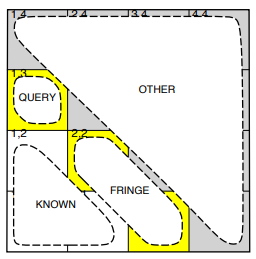
\includegraphics[]{images/wumpus-probs2.png}
\end{center}
The key insight is that the observed breezes are conditionally independent of the other variables, given the known, frontier, and query variables. To use the insight, we manipulate the query formula into a form in which the breezes
are conditioned on all the other variables, and then we apply conditional independence:
\begin{center}
    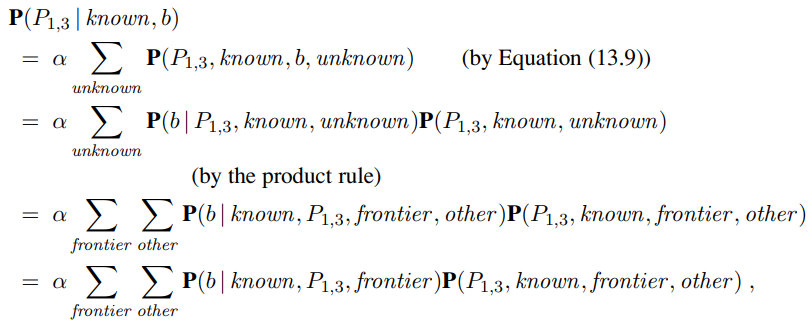
\includegraphics[]{images/wumpus-probs3.png}
\end{center}
where the final step uses conditional independence: $b$ is independent of $other$ given $known$, $P_{1,3}$, and $frontier$. Now, the first term in this expression does not depend on the $Other$ variables, so we can move the summation inward:
\begin{center}
    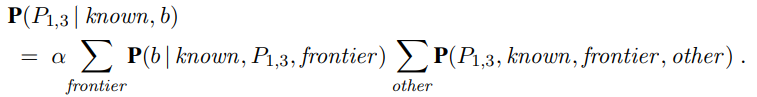
\includegraphics[]{images/wumpus-probs4.png}
\end{center}
By independence, as in Equation (1), the prior term can be factored, and then the terms can be reordered:
\begin{center}
    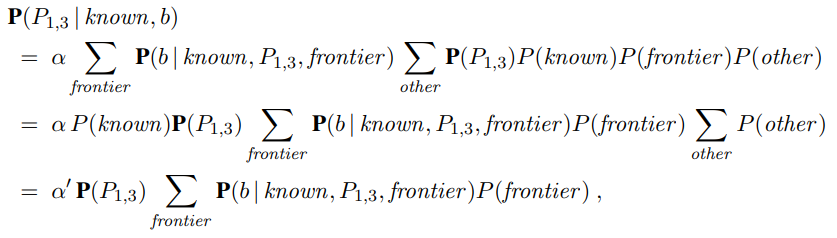
\includegraphics[]{images/wumpus-probs5.png}
\end{center}
where the last step folds $P(known)$ into the normalizing constant and uses the fact that $\sum_{other}P(other) = 1$. The use of independence and conditional independence has completely eliminated the other squares from consideration.\\\\
Notice that the expression $\textbf{P}(b | known, P_{1,3}, frontier )$ is 1 when the frontier is consistent with the breeze observations, and 0 otherwise. Thus, for each value of $P_{1,3}$, we sum over the logical models for the frontier variables that are consistent with the known facts.
\begin{center}
    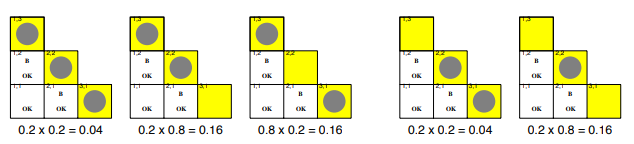
\includegraphics[]{images/wumpus-frontier.png}
\end{center}
Basically, we have that, when there is a pit in $[1,3]$, $frontier$ is either $p_{2,2} \land p_{3,1}$, or $p_{2,2} \land \neg p_{3,1}$ or $\neg p_{2,2} \land p_{3,1}$. $P(p_{2,2} \land p_{3,1}) = 0.2 \times 0.2$ because, by assumption, each square contains a pit with probability 0.2. For the same reason, $P(p_{2,2} \land \neg p_{3,1}) = 0.2 \times 0.8$ and $P(\neg p_{2,2} \land p_{3,1}) = 0.8 \times 0.2$ respectively. The same reasoning applies also for $\neg p_{1, 3}$ 
\\\\
Then, we have:
\[\textbf{P}(P_{1,3} | known, b) = \alpha ' <0.2(0.04 + 0.16 + 0.16), 0.8(0.04 + 0.16)> \approx <0.31, 0.69>\]
That is, $[1,3]$ (and $[3,1]$ by symmetry) contains a pit with roughly 31\% probability. A similar calculation shows that $[2,2]$ contains a pit with
roughly 86\% probability. The wumpus agent should definitely avoid $[2,2]$!

